\documentclass{article}
\usepackage[utf8]{inputenc}
\usepackage{amsmath}
\usepackage{amsfonts}
\usepackage{amssymb}
\usepackage[cm]{fullpage}
\usepackage{hyperref}
\usepackage{enumitem}
\usepackage{array}
\usepackage{graphicx}
\usepackage{float}
\usepackage{moreverb}
\setdescription{labelindent=\parindent}
\usepackage{algorithm}
%\usepackage{algorithmic}
\usepackage[noend]{algpseudocode}
\usepackage{mathtools}
\DeclarePairedDelimiter\ceil{\lceil}{\rceil}
\DeclarePairedDelimiter\floor{\lfloor}{\rfloor}
\begin{document}
\title
{\begin{flushleft}
\normalsize
Patrick Pegus\\
Homework 1\\
\today\\
CMPSCI-645\\
Prof. Meliou\\
Wenzhao Liu
\end{flushleft}}
\author{}
\date{}
\maketitle
In both plots, the near linear curves on the log-log scale suggest a power law relationship between $k$ and $f(k)$.
\begin{figure}[H]
	\centering
	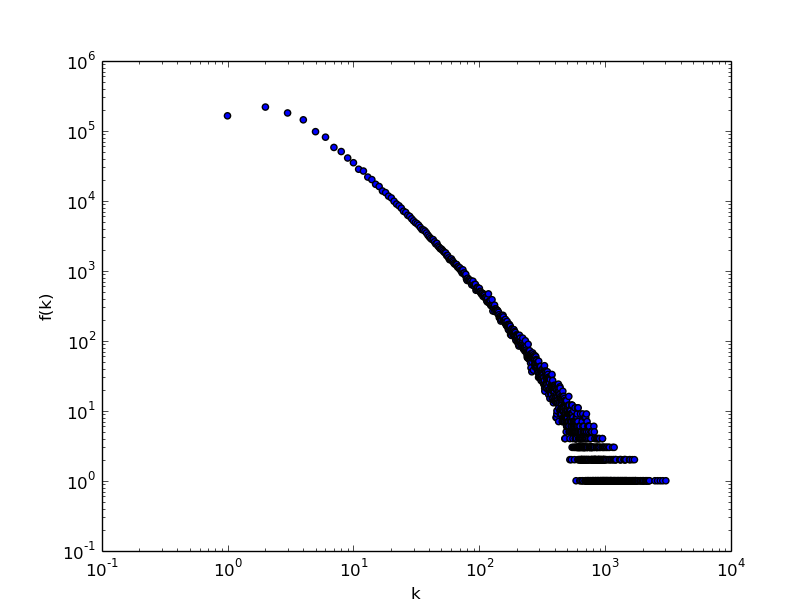
\includegraphics[width=0.5\textwidth]{collabcount.png}
	\caption{k = collaborator count, f(k) = number of authors having k collaborators}
\end{figure}
\begin{figure}[H]
	\centering
	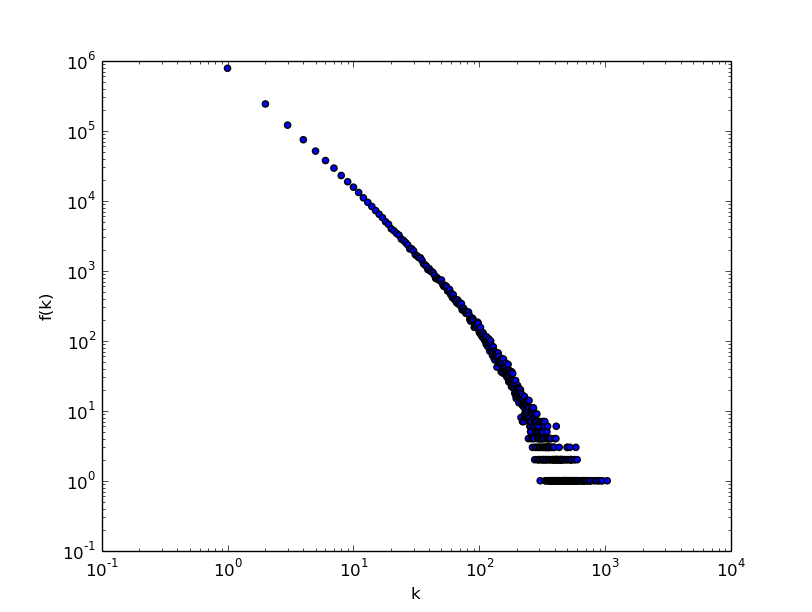
\includegraphics[width=0.5\textwidth]{pubcount.png}
	\caption{k = publication count, f(k) = number of authors having k publications}
\end{figure}
\end{document}
